\documentclass[pdflatex, sn-nature]{sn-jnl}

%%%% Standard Packages
%%<additional latex packages if required can be included here>

\usepackage{graphicx}%
\usepackage{multirow}%
\usepackage{amsmath, amssymb, amsfonts, cancel}%
\usepackage{amsthm}%
\usepackage[title]{appendix}%
\usepackage{xcolor}%
\usepackage{textcomp}%
\usepackage{manyfoot}%
\usepackage{booktabs}%
\usepackage{algorithm}%
\usepackage{algorithmicx}%
\usepackage{algpseudocode}%
\usepackage{listings}%
\usepackage{enumitem}%
\usepackage{tikz}%
\usepackage{xurl}%
\usetikzlibrary{bayesnet,positioning,fit,calc}%
\setlist[itemize]{leftmargin=1.5em,itemsep=0.2em,topsep=0.3em,parsep=0pt}

\theoremstyle{thmstyleone}%
\newtheorem{theorem}{Theorem}%
\newtheorem{proposition}[theorem]{Proposition}%

\theoremstyle{thmstyletwo}%
\newtheorem{example}{Example}%
\newtheorem{remark}{Remark}%

\theoremstyle{thmstylethree}%
\newtheorem{definition}{Definition}%

\setlength{\marginparwidth}{2cm}

\usepackage{multicol}

%%%% maths operators
% Sets
\newcommand \NN {\mathbb{N}}
\newcommand \ZZ {\mathbb{Z}}
\newcommand \QQ {\mathbb{Q}}
\newcommand \RR {\mathbb{R}}

% Indicator
\newcommand \indic {\mathbbm{1}}

% Probability Operators
\DeclareMathOperator*{\prob}{\mathbb{P}}
\DeclareMathOperator*{\esp}{\mathbb{E}}
\DeclareMathOperator*{\var}{\mathbb{V}\text{ar}}
\DeclareMathOperator*{\cov}{\mathbb{C}\text{ov}}
\newcommand \PP [1]{\prob\left({#1}\right)}
\newcommand \EE [1]{\esp\left[{#1}\right]}
\newcommand \VV [1]{\var\left[{#1}\right]}
\newcommand \CC [1]{\cov\left[{#1}\right]}
% Law
\newcommand \unif [1] {\mathcal{U}\left({#1}\right)}
\newcommand \normal [2] {\mathcal{N}\left({#1},{#2}\right)}

% Operators
\DeclareMathOperator*{\argmax}{arg\,max}
\DeclareMathOperator*{\argmin}{arg\,min}
% Matrix
\DeclareMathOperator*{\diag}{Diag}
\DeclareMathOperator*{\rank}{Rank}
\DeclareMathOperator*{\DET}{Det}
\DeclareMathOperator*{\Tr}{Tr}
\DeclareMathOperator*{\ES}{ES} 
\DeclareMathOperator*{\COV}{Cov}
\DeclareMathOperator*{\Spectrum}{Spectrum}

% To name R packages
\newcommand{\CRANpkg}[1]{\href{https://CRAN.R-project.org/package=#1}{\textbf{#1}}}
\newcommand{\strong}[1]{\texorpdfstring%
{{\normalfont\fontseries{b}\selectfont #1}}%
{#1}}
\newcommand{\code}[1]{\verb|#1|}

% Colours of the single-cell derivation (Appendix): technical scales and composition.
\definecolor{scalecol}{HTML}{C45C26}
\definecolor{compcol}{HTML}{1D4E89}


\raggedbottom

\begin{document}
    \title[DeCovarT: A Probabilistic and Multidimensional Framework for Cellular
    Deconvolution in Heterogeneous Biological Samples]{DeCovarT: A Probabilistic
    and Multidimensional Framework for Cellular Deconvolution in Heterogeneous Biological
    Samples}

    \author*[1,2]{\fnm{Bastien} \sur{Chassagnol}}
    \email{bastien\_chassagnol@laposte.net}
    \equalcont{B.C.\ and M.P.\ contributed equally to this work.}

    \author[3]{\fnm{Marielle} \sur{P\'{e}r\'{e}}}
    \email{marielle.pere@inria.fr}
    \equalcont{B.C.\ and M.P.\ contributed equally to this work.}

    \author[1]{\fnm{Mohamad} \sur{Al Charif}}

    \author[2]{\fnm{Gr\'{e}gory} \sur{Nuel}}
    \email{nuel@math.cnrs.fr}

    \author[4]{\fnm{Etienne} \sur{Becht}}
    \email{etienne.becht@inserm.fr}

    \author[1]{\fnm{Ana\"{i}s} \sur{Baudot}}
    \email{anais.baudot@univ-amu.fr}

    \affil[1]{\orgdiv{Marseille Medical Genetics (MMG), Systems Biomedicine team},
      \orgname{Aix-Marseille University, Inserm U1251},
      \orgaddress{\street{Facult\'{e} de M\'{e}decine, 27 Bd Jean Moulin},
        \city{Marseille}, \postcode{13385}, \country{France}}}

    \affil[2]{\orgdiv{Laboratoire de Probabilit\'{e}s, Statistique et
      Mod\'{e}lisation (LPSM), UMR 8001},
      \orgname{Sorbonne Universit\'{e} / CNRS},
      \orgaddress{\city{Paris}, \country{France}}}

    \affil[3]{\orgdiv{MacBes team},
      \orgname{Inria Centre at Universit\'{e} C\^{o}te d'Azur;
        Institut de Pharmacologie Mol\'{e}culaire et Cellulaire (IPMC)},
      \orgaddress{\city{Sophia-Antipolis}, \country{France}}}

    \affil[4]{\orgdiv{Centre de Recherche sur l'Inflammation (CRI),
      UMR 1149},
      \orgname{Inserm / Universit\'{e} Paris Cit\'{e}},
      \orgaddress{\street{Facult\'{e} de m\'{e}decine -- site Bichat,
        16 rue Henri Huchard},
        \city{Paris}, \postcode{75018}, \country{France}}}


        \abstract{%
        \textbf{Introduction.}
        Bulk transcriptomes have contributed to the characterisation of
        biological systems.
        Mechanisms are harder to separate, because signals from different
        cells are added in one measurement: a shift in cell-type composition
        and a fluctuation in the micro-environment are then confounded.
        Single-cell assays separate those signals.
        They remain costly and difficult to run at cohort scale.
        Deconvolution recovers the cell-type composition of a bulk profile
        from reference profiles, often built from single-cell RNA-seq.
        Current methods still fail when closely related types share similar
        expression.
        We hypothesise that a gene-regulatory network for each type can
        separate them.

        \textbf{Methods.}
        DeCovarT is a generative model of the bulk profile given latent
        cell-type-specific expression and the composition, with those
        networks in the covariance.
        Reference profiles supply a mean for each population.
        Gene--gene dependence in a cell type is a multivariate Gaussian
        precision, estimated by the graphical lasso.
        Weights on the \(\ell_{1}\) penalty can carry mechanistic prior
        knowledge.
        The bulk is the sum of the cell-type contributions, each weighted
        by its relative abundance.
        A cell type is not a fixed profile: its expression is drawn from
        that Gaussian.
        Independent populations make the bulk a weighted convolution, itself
        multivariate Gaussian.
        The likelihood supplies asymptotic confidence intervals for the
        estimated parameters.
        Figure~\ref{fig:overview} is a visual summary.

        \textbf{Results.}
        In a toy model, overlap between cell-type profiles was changed by
        changing only the gene--gene correlations.
        Larger overlap lowered the accuracy of standard deconvolution,
        including quadratic programming as in \emph{DeconRNASeq}.
        DeCovarT had lower error than those methods in the scenarios we
        evaluated.
        A planned extension uses \emph{SimBu} to build pseudo-bulk samples
        by drawing single-cell profiles in chosen proportions.

        \textbf{Use-case.}
        Organoids are three-dimensional structures grown from stem cells
        and used to model organ development and function.
        Differentiation still varies widely, including among organoids from
        isogenic lines kept on the same protocol.
        Bulk RNA-seq is often used to follow maturation over time, and that
        average hides cell-type-specific expression.
        A preliminary implementation of DeCovarT is applied to gastruloids,
        organoids that recapitulate early embryonic stages.
        The estimated proportions define a time-dependent potency score:
        how far the pluripotent cells present at that snapshot can still
        give rise to mature cell types.

        \textbf{Code and resources.}
        Theory, graphical models, and derivations:
        \url{https://cnrs.hal.science/hal-04208010}.
        The R package:
        \url{https://github.com/bastienchassagnol/DeCovarT}.
        }

        \keywords{deconvolution, bulk RNA-seq, weighted multivariate Gaussian distribution, covariance-driven model}

    \maketitle

\section{Introduction}
\label{sec:intro}

\subsection{Bulk versus single-cell}
\label{sec:context}

\begin{itemize}
  \item bulk RNA-seq: one profile per sample, summed over every cell present at that time
  \item that sum hides cell-specific signal
  \item two losses follow
  \begin{itemize}
    \item specificity: a shift in cell fractions read as differential expression
    \item sensitivity: genes of a minor type masked by a variable major type
  \end{itemize}
  \item gastruloids: morphotypes diverge along a trajectory of lineage fractions
        and cell states, even among structures from the same protocol
        \cite{suppingerMultimodalCharacterizationMurine2023}
  \item bulk time series: many gastruloids and many time points, one lysate each
  \begin{itemize}
    \item a stalled lineage, a changed mix of germ layers, and a
          micro-environmental shift are the same change in the average
    \item the morphotype is seen, the cell population that drove it is not
  \end{itemize}
  \item single-cell RNA-seq: types, states, and within-type spread at one snapshot
  \begin{itemize}
    \item names the driver: a missing lineage, a stalled state, or extra
          variance inside a type
    \item dissociation ends that gastruloid, and each gastruloid yields few
          cells, so the same structure cannot be followed through time
  \end{itemize}
  \item deconvolution: fractions from bulk, using a purified or single-cell reference
  \begin{itemize}
    \item the reference names the populations; repeated bulk then traces
          their fractions along the morphotype trajectory
  \end{itemize}
  \item published engines still fail when mean profiles nearly coincide,
        and most return only a point estimate of \(\boldsymbol{p}\)
\end{itemize}

\subsection{Review of alternative deconvolution methods}
\label{sec:gap}

\begin{itemize}
  \item most engines treat the signature as a fixed mean matrix
  \item gene--gene dependence inside each type is omitted
  \item regression and many machine-learning fits return a point \(\hat{\boldsymbol{p}}\) only
  \item \emph{CIBERSORT}: \(\nu\)-SVR on a mean signature; genes treated as independent
        \cite{newmanRobustEnumerationCell2015,newmanDeterminingCellType2019}
  \item \emph{DeconRNASeq}: non-negative least squares on the same mean map
        \cite{gongDeconRNASeqStatisticalFramework2013,dessoleLawsonHansonAlgorithmDeviation2023}
  \item \emph{DSection}: Bayesian univariate Gaussian convolution
        \cite{erkkilaProbabilisticAnalysisGene2010}
  \item \emph{DeMix} / \emph{DeMixT}: frequentist Gaussian mixture, independent genes,
        one unknown component
        \cite{ahnDeMixDeconvolutionMixed2013,wangTranscriptomeDeconvolutionHeterogeneous2018}
  \item \emph{RNA-Sieve}: gene-wise central-limit Gaussian, noisy reference, independent genes;
        Wald or Godambe intervals
        \cite{erdmann-phamLikelihoodbasedDeconvolutionBulk2021}
  \item \emph{MuSiC}: cross-sample means, dropout, protocol shift; still a mean-weighted regression
        \cite{wangBulkTissueCell2019}
  \item \emph{DWLS}: dampened gene weights on the mean residual
        \cite{tsoucasAccurateEstimationCelltype2019}
  \item \emph{DECALS}: decorrelated constrained least squares;
        sampling distribution of \(\hat{\boldsymbol{p}}\) under a subject-specific bulk covariance
        \cite{caiStatisticalInferenceCelltype2024}
  \item \emph{MEAD}: errors-in-variables intervals when gene-specific platform scales
        are unknown; identifiability of \(\boldsymbol{p}\) under those scales
        \cite{xieStatisticalInferenceCell2026}
  \item joint estimation of \(\boldsymbol{p}\) and \(\{\boldsymbol{\Sigma}_{j}\}\) from the same bulks
        is weakly identified
  \item DeCovarT keeps \((\boldsymbol{\mu},\{\boldsymbol{\Sigma}_{j}\})\) as a plug-in and estimates \(\boldsymbol{p}\) only
\end{itemize}

\subsection{DeCovarT}
\label{sec:decovart}

\begin{itemize}
  \item First innovation: model cell-type specific variability with a multivariate Gaussian convolution
  \item Second innovation: model the cell-type composition with a constrained maximum likelihood approach on the isometric log-ratio chart
  \cite{egozcueIsometricLogratioTransformations2003}
  \item Thrid innnovation: deive theroetical intervals to assess the gain of accuracy when 
  accounting for the cell-type specific variability compared to a mean-only approach. In addition, proposes
  new asymtotic tests to evaluate the absnce or presence of one or several cell proportions (referred to as active null
  cell types).
\end{itemize}

\begin{itemize}
      \item A new modelling and versatile framework to test the impact of the covariance structure on the deconvolution performance
\begin{itemize}
      \item Gram matrix decompsotion to target the cosine of the mean profiles.
      \item Use a variety of random network topologies to parametrize the covariance structure.
      \item MixSim average overlap of the purified Gaussians: misassignment probability
            of a labelled cell, hence a lower bound on compositional error
            \cite{melnykovMixSimPackageSimulating2012,rianiSimulatingMixturesMultivariate2015}
     \item normalised Shannon entropy of \(\boldsymbol{p}\)
     
          \end{itemize}
\end{itemize}

\section{Results}
\label{sec:results}

\subsection{Overview}
\label{sec:overview}

\begin{itemize}
  \item Figure~\ref{fig:overview}: generative model, bulk constructions, and the linear mixture
  \item Figure~\ref{fig:scenarios}: synthetic means, precision graphs, overlap, and scores
  \item claim to test: a shared mean is not enough to separate close types
  \item larger effect expected on interval coverage than on point bias
  \item separation is possible when means match and precision graphs do not
  \item rare types: wide intervals; pool them, or treat them as a residual component
  \item reporting frame: ADEMP (bias, RMSE, coverage, failure), no default composite score
        \cite{morrisUsingSimulationStudies2019}
\end{itemize}

\begin{figure}[tbp]
  \centering
  \includegraphics[width=\textwidth]{"figs/Figure 1_ DeCovarT overview.png"}
  \caption{Overview of DeCovarT.
    Top: plate diagram.
    The soft-max map \(\psi\) sends \(\boldsymbol{\rho}_{i}\) to a composition \(\boldsymbol{p}_{i}\).
    Latent profiles \(\boldsymbol{x}_{\cdot j}\) are independent
    \(\mathcal{N}(\boldsymbol{\mu}_{j},\boldsymbol{\Sigma}_{j})\).
    The bulk is the mixture \(\boldsymbol{y}_{i}=\boldsymbol{X}\boldsymbol{p}_{i}\)
    and, marginally, the Gaussian convolution.
    Bottom left: three ways to build a bulk
    (one population; shared cell-size ratios; library-size ratios),
    and the further assumption required before \(\boldsymbol{p}\) is a cell fraction.
    Bottom centre: three types, with RNA content \(\mu_{g}\) times cell fraction \(p_{j}\).
    Bottom right: reference means and gene-regulatory graphs, the bulk matrix,
    and the same linear reconstruction.}
  \label{fig:overview}
\end{figure}

\begin{figure}[tbp]
  \centering
  \includegraphics[width=\textwidth]{"figs/Figure 2_ the synthetic simulation framework.jpg"}
  \caption{Synthetic simulation framework.
    Panel~A, left to right and top to bottom:
    Gram--Schmidt / spectral construction of the mean profiles;
    stochastic block model and Barab\'asi--Albert precision graphs;
    Shannon entropy of \(\boldsymbol{p}\) across six types;
    overlap of two purified Gaussians (linear and quadratic decision boundaries).
    Panel~B: root-mean-square error, Aitchison distance on the simplex,
    and the split between theoretical failure of the likelihood and numerical failure of the solver.}
  \label{fig:scenarios}
\end{figure}

\subsection{Bivariate toy: two genes, two cell types}
\label{sec:bivariate}


\begin{itemize}
  \item purpose: check that gene--gene correlation changes the estimated fractions
        when only two genes and two cell types are observed
  \item one free isometric log-ratio coordinate on the simplex;
        the likelihood is a curve, then mapped back to \(\boldsymbol{p}\)
  \item each purified profile is Gaussian;
        the bulk is their abundance-weighted sum, with no extra noise
        \eqref{eq:convolution}
  \item \(G=2\), \(J=2\), \(N=500\) Monte Carlo bulks per scenario, \(972\) scenarios
  \item composition \(\boldsymbol{p}\): balanced \((1/2,1/2)\),
        moderately unbalanced \((17/20,3/20)\),
        highly unbalanced \((99/100,1/100)\)
  \item centroid gap: small, \(\boldsymbol{\mu}_{\cdot 1}=(20,22)\) versus
        \(\boldsymbol{\mu}_{\cdot 2}=(22,20)\);
        large, \((20,40)\) versus \((40,20)\)
  \item within-type correlation \(\rho_{j}\in\{-0.8,-0.6,\ldots,0.8\}\),
        set separately for each type
  \item marginal variances: equal, \((1,1)\), or unequal, \((1,2)\)
  \item solvers: NNLS; \emph{DeconRNASeq} (\texttt{lsei}); L-BFGS-B; projected gradient;
        Newton--Raphson; Marquardt--Levenberg; simulated annealing
  \item mean-only solvers minimise \(\|\boldsymbol{y}-\boldsymbol{\mu}\boldsymbol{p}\|^{2}\)
        and carry no convolution Wald standard error
  \item script
        \url{https://github.com/bastienchassagnol/DeCovarT/blob/main/scripts/fig02_bivariate_toy.R}
  \item vignette
        \url{https://bastienchassagnol.github.io/DeCovarT/articles/fig02-bivariate-toy.html}
  \item books
        \url{https://github.com/bastienchassagnol/DeCovarT/tree/main/output/fig02}
  \item file-by-file reading: Appendix~\ref{app:fig02}
\end{itemize}

\begin{figure}[tbp]
  \centering
  \includegraphics[width=\textwidth]{"figs/Figure 3, panel A.png"}
  \caption{Bivariate toy, panel~A.
    Centre: root-mean-square error on the \((\rho_{1},\rho_{2})\) grid
    (colour scale about \(0.10\) to \(0.20\)).
    Four insets: two-gene mixture densities at correlation corners,
    with \(95\%\) ellipses of the purified types.
    Outer panels: Monte Carlo \(\hat{\boldsymbol{p}}\) as dot-whisker forests
    and as rainclouds, for Newton--Raphson, Marquardt--Levenberg, L-BFGS, and projected gradient.
    Black squares and arrows mark which grid cell each density belongs to.}
  \label{fig:bivariate}
\end{figure}

\subsection{Covariance-driven scenario: twenty genes, three cell types}
\label{sec:hd}

\begin{itemize}
  \item role: mean-collinear types, discriminative signal moved into the precision graphs
  \item script
        \url{https://github.com/bastienchassagnol/DeCovarT/blob/main/scripts/fig03_variance_driven.R}
  \item vignette
        \url{https://bastienchassagnol.github.io/DeCovarT/articles/fig03-covariance-driven.html}
  \item books
        \url{https://github.com/bastienchassagnol/DeCovarT/tree/main/output/fig03}
  \item file-by-file reading: Appendix~\ref{app:fig03}
  \item \(G=20\), \(J=3\), \(N=50\) bulks per scenario, \(36\) scenarios, seed \texttt{20260807}
  \item one Gram: cosines \(0.9\) (types 1--2) and \(0.1\) (either of those versus type 3); scale \(s=10\)
  \item types 1 and 2: scale-free or cluster stochastic block model, \(2\times 2\) assignments
        \cite{barabasiEmergenceScalingRandom1999,hollandStochasticBlockmodelsFirst1983}
  \item type 3: scale-free, held fixed
  \item covariance scale chosen so MixSim average overlap hits \(0.02\), \(0.08\), or \(0.20\)
  \item overlap matched at the balanced composition; unbalanced \(\boldsymbol{p}\) raises the realised overlap
  \item compositions from normalised Shannon entropy \(H^{\star}\in\{1,0.5,0.1\}\)
  \item solvers: \emph{DeconRNASeq} (\texttt{lsei}); \emph{CIBERSORT}; L-BFGS-B;
        Newton--Raphson; Marquardt--Levenberg
\end{itemize}

\begin{figure}[tbp]
  \centering
  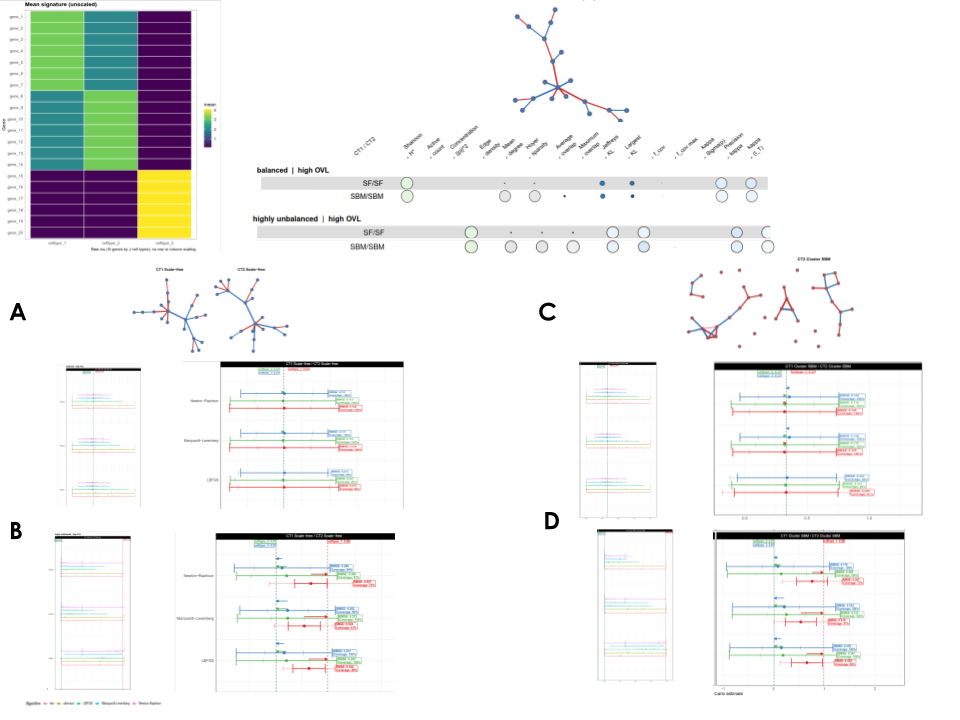
\includegraphics[width=\textwidth]{figs/Fig4_HD_framework.png}
  \caption{Covariance-driven scenario.
    Top left: unscaled mean signature \(\boldsymbol{\mu}\);
    types 1 and 2 share the high-cosine block, type 3 carries the contrasting block.
    Networks: scale-free and stochastic-block skeletons.
    Two descriptor strips, both at high overlap:
    balanced composition, then highly unbalanced composition
    (Shannon entropy, overlap, conditioning, divergences; SF/SF and SBM/SBM rows).
    Forests: ADEMP summaries for those two regimes.
    Solver colours: \texttt{lsei}, \emph{CIBERSORT}, L-BFGS-B,
    Marquardt--Levenberg, Newton--Raphson.
    Solid whiskers use the expected-Fisher Wald standard error;
    dashed whiskers use the Monte Carlo standard deviation.}
  \label{fig:hd}
\end{figure}

\subsection{Planned biological application}
\label{sec:gastruloid}

\begin{itemize}
  \item dataset: murine gastruloids, multimodal characterisation
        \cite{suppingerMultimodalCharacterizationMurine2023}
  \item batch-to-batch viability and morphotype vary under matched protocols
  \item developmental states form a potency gradient, unlike discrete blood lineages
  \item comparison set: DeCovarT against mean-only engines on the same genes and the same reference
  \item not yet run
\end{itemize}

\subsection{Planned robustness}
\label{sec:robustness}

\begin{itemize}
  \item extra diagonal bulk noise on top of \(\boldsymbol{\Sigma}(\boldsymbol{p})\)
  \item counts that are not Gaussian (negative binomial, Poisson--log-normal)
        \cite{chiquetPoissonLognormalModelVersatile2021,wangBulkTissueCell2019}
  \item dropout, as in \emph{MuSiC} \cite{wangBulkTissueCell2019}
  \item a reference that omits one type \cite{wangBulkTissueCell2019}
  \item protocol shift between the reference and the bulk \cite{wangBulkTissueCell2019}
  \item vignette
        \url{https://bastienchassagnol.github.io/DeCovarT/articles/supp-S5-misspecification.html}
\end{itemize}

\section{Methods}
\label{sec:methods}

\subsection{Notation}
\label{sec:notation}

Bulk sample \(i\) is fixed inside a derivation.
The index \(i\) is restored in the model statements.
Base indices used throughout: gene \(g=1,\ldots,G\), cell type \(j=1,\ldots,J\),
sample \(i=1,\ldots,N\).
Table~\ref{tab:notation} is the alignment layer
(\url{https://bastienchassagnol.github.io/DeCovarT/articles/theory-decovart-single-cell-bulk-alignment.html}).

\begin{table}[tbp]
  \centering
  \caption{Cell counts, scales, and the two covariance mixtures.
    \(\boldsymbol{\rho}\) elsewhere in the paper is the isometric log-ratio
    coordinate of \(\boldsymbol{p}\), so the within-type correlation is \(\varrho\).}
  \label{tab:notation}
  \begin{tabular}{@{}lp{0.62\textwidth}@{}}
    \toprule
    Symbol & Meaning \\
    \midrule
    \(m_{ji}\in\mathbb{N}\) &
      Number of cells of type \(j\) in bulk sample \(i\)
      (\emph{MuSiC} writes \(m_{kj}\)). \\
    \(n_{i}=\sum_{j}m_{ji}\) &
      Total number of cells in bulk sample \(i\). \\
    \(\boldsymbol{m}_{\cdot i}=(m_{1i},\ldots,m_{Ji})^{\top}\) &
      Cell-count vector; \(\boldsymbol{p}_{\cdot i}=\boldsymbol{m}_{\cdot i}/n_{i}\). \\
    \(\kappa_{i}=1/n_{i}\) &
      Per-cell averaging factor. \\
    \(\boldsymbol{w}_{\cdot i}=a_{i}\boldsymbol{m}_{\cdot i}\) &
      Effective counts on the bulk molecule scale. \\
    \(\boldsymbol{D}_{i}=\boldsymbol{\Sigma}_{\mathrm{obs},i}
      =\operatorname{diag}(\tau_{1i}^{2},\ldots,\tau_{Gi}^{2})\) &
      Diagonal, heteroscedastic bulk measurement noise. \\
    \(\boldsymbol{T}_{ji}=\sum_{c=1}^{m_{ji}}\boldsymbol{X}_{jic}\) &
      Total expression contributed by type \(j\) to sample \(i\). \\
    \(\boldsymbol{S}_{W}(\boldsymbol{v})=\sum_{j}v_{j}\boldsymbol{\Sigma}_{W,j}\) &
      Linear covariance mixture with weights \(\boldsymbol{v}\). \\
    \(\boldsymbol{S}_{B}(\boldsymbol{v})=\sum_{j}v_{j}^{2}\boldsymbol{\Sigma}_{B,j}\) &
      Quadratic covariance mixture. \\
    \(\varrho_{j}\in[-1/(m_{ji}-1),1]\) &
      Cell-to-cell correlation inside type \(j\). \\
    \(\boldsymbol{\vartheta}\) &
      Generic parameter vector;
      \(\boldsymbol{\theta}_{\cdot j}\) keeps the meaning of relative abundance. \\
    \(\boldsymbol{\mu}_{k},\boldsymbol{\Sigma}_{k},
      \boldsymbol{\mu}_{kl},\boldsymbol{\Sigma}_{kl}\) &
      First and second partial derivatives of the mean and covariance
      in \(\vartheta_{k},\vartheta_{l}\). \\
    \bottomrule
  \end{tabular}
\end{table}

\subsection{Generative model}
\label{sec:model}

\begin{itemize}
  \item ideal model in this section: no platform scale yet (alignment is \S\ref{sec:alignment})
  \item latent profile \(\boldsymbol{x}_{\cdot j,i}\sim\mathcal{N}(\boldsymbol{\mu}_{\cdot j},\boldsymbol{\Sigma}_{j})\)
  \item bulk \(\boldsymbol{y}_{\cdot i}=\sum_{j}p_{ji}\,\boldsymbol{x}_{\cdot j,i}\)
  \item implied law, the estimating equation of DeCovarT
  \item derivatives, ILR chain rule, and Fisher information
        \url{https://bastienchassagnol.github.io/DeCovarT/articles/theory-decovart-generative-model.html}
\end{itemize}

\begin{equation}
  \boldsymbol{y}_{\cdot i}
  \sim
  \mathcal{N}\!\left(
    \boldsymbol{\mu}\boldsymbol{p}_{\cdot i},\;
    \sum_{j=1}^{J} p_{ji}^{2}\,\boldsymbol{\Sigma}_{j}
  \right)
  \label{eq:convolution}
\end{equation}

\begin{itemize}
  \item the factor \(p_{ji}^{2}\) is the variance of a sum of independent types
  \item plug-in \((\boldsymbol{\mu},\{\boldsymbol{\Sigma}_{j}\})\); unknown is \(\boldsymbol{p}_{\cdot i}\) only
  \item \(\boldsymbol{S}_{B}(\boldsymbol{p}_{\cdot i})\) in Table~\ref{tab:notation} is this quadratic mixture
        when the weights are the cell fractions
  \item sparse \(\boldsymbol{\Omega}_{j}=\boldsymbol{\Sigma}_{j}^{-1}\) may be supplied by a Gaussian Markov graph
        \cite{friedmanSparseInverseCovariance2008,chiquetVariationalInferenceSparse2018}
\end{itemize}

\subsection{Inference}
\label{sec:inference}

\begin{itemize}
  \item objective: Gaussian log-likelihood of \eqref{eq:convolution}
  \item default chart: isometric log-ratio, a \(C^{2}\) diffeomorphism of the open simplex
        \cite{egozcueIsometricLogratioTransformations2003}
  \item additive log-ratio kept as an appendix chart, not the default
  \item L-BFGS-B: box constraints in \(\boldsymbol{p}\), then renormalise
        \cite{byrdLimitedMemoryAlgorithm1995}
  \item Newton--Raphson: analytic Hessian in isometric log-ratio coordinates
  \item Marquardt--Levenberg: damped Newton (\texttt{marqLevAlg}),
        stop on the relative distance to the maximum
        \cite{marquardtAlgorithmLeastSquaresEstimation1963,philippsRobustEfficientOptimization2021,commengesNewtonLikeAlgorithmLikelihood2006}
  \item the log-likelihood is not concave; a local maximum is not certified global
  \item interior interval: Wald standard error from the expected Fisher information,
        delta method back to \(\boldsymbol{p}\)
  \item one bulk column is an \(N=1\) fit: the interval describes that maximiser
  \item on a face of the simplex the likelihood-ratio null is chi-bar-square, not \(\chi^{2}\)
        \cite{selfAsymptoticPropertiesMaximum1987}
  \item full argument
        \url{https://bastienchassagnol.github.io/DeCovarT/articles/theory-DeCovarT-MLE-properties.html}
\end{itemize}

\subsection{Synthetic scenarios}
\label{sec:synthetic}

\begin{itemize}
  \item pipeline
        \url{https://bastienchassagnol.github.io/DeCovarT/articles/theory-synthetic-scenarios-mean-covariance.html}
  \item means: orthonormal frame times a Gram square root, optional non-negativity
        (Figure~\ref{fig:scenarios}A)
  \item graphs: scale-free preferential attachment, stochastic block model;
        precision shifted to be positive definite
  \item overlap: global covariance scale, support of \(\boldsymbol{\Omega}_{j}\) held fixed
  \item descriptors to report with every scenario
  \begin{itemize}
    \item Shannon entropy of \(\boldsymbol{p}\)
    \item cosine and Euclidean centroid gap of \(\boldsymbol{\mu}\)
    \item MixSim average overlap of the purified components
    \item condition number of \(\boldsymbol{\Sigma}(\boldsymbol{p})\)
    \item fraction of tangent Fisher information carried by the covariance block
    \item edge density of each precision graph
  \end{itemize}
  \item scores: Euclidean and Aitchison error on \(\boldsymbol{p}\); RMSE; MAE; bias;
        coverage with a Wilson interval; optimiser failure
        \cite{morrisUsingSimulationStudies2019}
  \item do not collapse those scores into one weighted index unless the weights are shown beside it
\end{itemize}

\subsection{Reference alignment and the gastruloid cohort}
\label{sec:alignment}

\subsubsection{Suppinger gastruloids}

\begin{itemize}
  \item source: multimodal murine gastruloid characterisation
        \cite{suppingerMultimodalCharacterizationMurine2023}
  \item to extract: batches, viability, annotated states, matched bulk if any
  \item status: not yet analysed in this repository
\end{itemize}

\subsubsection{Which genes enter the signature}

\begin{itemize}
  \item aim: genes that separate close types, using means and variances
  \item one biological replicate: the sample covariance is unstable; use a structured precision
  \item several biological replicates: cross-sample covariance of pseudobulk or sorted profiles
  \item three reference regimes
        \url{https://bastienchassagnol.github.io/DeCovarT/articles/theory-decovart-statistical-perspectives.html}:
        sorted populations; one single-cell replicate;
        enough replicates to split within-type and between-replicate covariance
\end{itemize}

\subsubsection{Platform scale}

Three strategies, written out in
\url{https://bastienchassagnol.github.io/DeCovarT/articles/theory-decovart-single-cell-bulk-alignment.html}.

\begin{itemize}
  \item cell-count convolution: covariance linear in \(m_{ji}\)
        (\(\boldsymbol{S}_{W}\) in Table~\ref{tab:notation})
  \item averaged mixture: profile per cell, library size kept as a scale \(\kappa_{i}\)
  \item library-size closure (TPM, RPKM): gene fractions on a simplex
  \item working position on absolute cell counts: capture efficiency is not observed
  \item working position on library-size closure: dividing by the total induces
        gene--gene correlation, including for genes that were independent
  \item estimand under \eqref{eq:convolution}: relative transcriptomic contribution
  \item that contribution equals the cell fraction only if capture and RNA content per cell
        are shared across types
        \cite{racleSimultaneousEnumerationCancer2017}
  \item both equalities are unlikely for gastruloid states; state the estimand next to \(\hat{\boldsymbol{p}}\)
\end{itemize}

\section{Discussion and Perspectives}
\label{sec:perspectives}

\subsection{DeCovarT's limitations}
\label{sec:limitations}

\begin{itemize}
  \item cell-type composition: a relevant prognostic biomarker of gastruloid fate
  \item single-cell RNA-seq: abnormal cell states, at higher resolution than bulk
  \item cost and technical burden limit large-scale studies with enough power
  \item dissociation destroys the organoid, and each organoid has few cells,
        so the same organoid cannot be followed across time points
  \item DeCovarT collects, in one likelihood, ideas from algorithms that
        model within-cell-type variability
  \begin{itemize}
    \item \emph{MuSiC}: one scale aligns the bulk average with the single-cell
          average, for library size and capture efficiency across platforms
          \cite{wangBulkTissueCell2019}
    \item \emph{RNA-Sieve}: cell-type profiles as Gaussian.
          With enough single cells, a central-limit argument applies to the
          moments (mean and variance), even when the observations themselves
          are not Gaussian.
          DeCovarT drops the assumption that genes are independent
          \cite{erdmann-phamLikelihoodbasedDeconvolutionBulk2021}
    \item \emph{DECALS}: joint estimate of the composition and of the
          cell-type covariances, so both within-type and cross-sample
          variability enter the fit
          \cite{caiStatisticalInferenceCelltype2024}
    \item \emph{MEAD}: an errors-in-variables Gaussian model, and confidence
          intervals for the estimated proportions
          \cite{xieStatisticalInferenceCell2026}
  \end{itemize}
  \item benchmarks that cross algorithms with normalisation choices:
        raw counts as the proxy of mRNA abundance
  \item library-size normalisations such as TPM turn the problem into a
        composition on the gene simplex
  \item the scaling assumptions in Figure~\ref{fig:overview} are unlikely
        to hold; absolute mRNA content per cell type then needs an external
        reference or an orthogonal assay
  \item estimand: share of transcriptomic content per cell type, not the
        cell-count composition
\end{itemize}

\subsection{Other observation laws and inverse problems}
\label{sec:outlook}

\begin{itemize}
  \item \emph{RNA-Sieve}, \emph{MEAD}, and \emph{DECALS} support a
        multivariate Gaussian model for the genes, and only asymptotically
  \item none of the three states a lower bound on the number of single-cell
        profiles per cell type
  \item with few profiles, a logit-normal law can give better-calibrated
        intervals
        \cite{mcgregorProportionalitybasedAssociationMetrics2026}
  \item multivariate counts rarely have a closed form
        (negative-binomial or log-normal margins)
  \item a convolution under those laws needs numerical integration or
        Monte Carlo
\end{itemize}

Alternative distributions already used for deconvolution:

\begin{itemize}
  \item discrete counts: \emph{ISOpureR}, \emph{BayesPrism} (multinomial)
        \cite{anghelISOpureRImplementationComputational2015,chuCellTypeGeneExpression2022};
        \emph{DeconV} (Poisson) \cite{gynterDeconvProbabilisticCellType2023};
        Poisson--log-normal and zero-inflated extensions
        \cite{chiquetPoissonLognormalModelVersatile2021,batardiereZeroInflationMultivariatePoisson2025};
        \emph{RCTD} \cite{cableRobustDecompositionCell2022a}
  \item continuous, gene-wise: \emph{BLADE} (log-normal, variational cell-type profiles)
        \cite{andrade-barbosaBayesianLogNormalDeconvolution2021};
        \emph{bMIND} \cite{wangBayesianEstimationCelltypespecific2020}
  \item once \(\boldsymbol{p}_{\cdot i}\) is known, the conditional mean of \(\boldsymbol{x}_{\cdot j,i}\)
        is the MAP, the BLUP, and the Wiener filter of the Gaussian convolution
  \item \emph{CSNet} reverses \eqref{eq:convolution}: \(\boldsymbol{p}\) treated as known,
        type-level means and a sparse correlation estimated by least squares
        \cite{suEstimatingCellTypeSpecificGene2024}
  \item a \emph{CSNet} correlation is a co-expression graph;
        a graphical lasso on \(\hat{\boldsymbol{\Sigma}}_{j}\) is the precision
        DeCovarT can plug in
        \cite{friedmanSparseInverseCovariance2008}
\end{itemize}

\subsection{Regulatory networks from single-cell profiles}
\label{sec:grn}

Beside the mean of each cell type, DeCovarT needs
\(\boldsymbol{\Sigma}_{j}\) or \(\boldsymbol{\Omega}_{j}\).
Gene--gene dependence estimated from single cells is still an open problem.

\begin{itemize}
  \item the fitted precision is undirected; most regulatory interactions are directed
  \begin{itemize}
    \item orient edges by pairing observations with interventions
    \item or add chromatin accessibility, or transcription-factor binding
          \cite{badia-i-mompelGeneRegulatoryNetwork2023,maizelsGeneRegulatoryNetworks2026}
  \end{itemize}
  \item open question: whether a causal graph improves \(\hat{\boldsymbol{p}}\),
        or a consistent covariance is enough
  \item current fits use the variability inside one single-cell biological replicate
  \item several independent replicates would separate that within-type term
        from cross-sample variability, for example with a two-level
        hierarchical random effect
  \item \emph{DECALS} already splits those two variance layers;
        DeCovarT does not implement that split yet
        \cite{caiStatisticalInferenceCelltype2024}
\end{itemize}



\begin{appendices}
\section{Bivariate plot books}
\label{app:fig02}

Directory of the \(G=2\), \(J=2\) books
(\(N=500\) bulks, \(972\) scenarios):

\url{https://github.com/bastienchassagnol/DeCovarT/tree/main/output/fig02}

Density pages under \texttt{density\_visualisations/}.
Shared corners
\((\rho_{1},\rho_{2})\in\{(0,0),(-0.8,-0.8),(0.8,0.8),(-0.8,0.8)\}\),
twelve meta-scenarios (centroid gap \(\times\) variance \(\times\) composition).

\begin{itemize}
  \item \texttt{purified\_density.pdf}: the two cell-type Gaussians before mixing
  \item \texttt{bulk\_density.pdf}: the convolution that DeCovarT fits
  \item \texttt{loglik\_surface\_p.pdf}: log-likelihood of one bulk on the simplex;
        colour is \(\log_{10}(L/\max L)\)
  \item \texttt{loglik\_ilr\_profile.pdf}: the same surface as a curve in the
        single isometric log-ratio coordinate
  \item \texttt{loglik\_expected\_surface\_p.pdf},
        \texttt{loglik\_expected\_ilr\_profile.pdf}:
        expected log-likelihood at the true \(\boldsymbol{p}\), not one draw
  \item \texttt{loglik\_rgl.pdf}: the same relative likelihood as a 3D surface;
        white marker at \(\boldsymbol{p}^{\star}\), red marker at the numerical maximum
\end{itemize}

Performance pages under \texttt{performance\_visualisations/}.

\begin{itemize}
  \item \texttt{heatmap\_rmse.pdf}, \texttt{heatmap\_mae.pdf},
        \texttt{heatmap\_aitchison.pdf}:
        tiles on \((\rho_{1},\rho_{2})\); one page per meta-scenario; seven solver panels
  \item \texttt{forest.pdf}: ADEMP dot-whisker for the convolution solvers
        \cite{morrisUsingSimulationStudies2019,allenRaincloudPlotsMultiplatform2019}
  \begin{itemize}
    \item solid whisker: \(1.96\) times the expected-Fisher Wald standard error
          at the true composition
    \item dashed whisker: empirical Monte Carlo standard deviation
    \item labels: RMSE and coverage of that cell type
  \end{itemize}
  \item \texttt{raincloud.pdf}: full Monte Carlo law of \(\hat{p}\),
        including pile-up at \(0\) and \(1\)
  \item \texttt{dotsinterval.pdf}: the same quantiles without a kernel density on \([0,1]\)
  \item \texttt{qq\_normal.pdf}: whitened isometric log-ratio coordinate against \(N(0,1)\)
  \item \texttt{qq\_chi2.pdf}: squared Mahalanobis distance against \(\chi^{2}_{1}\)
  \item \texttt{ks\_normal.pdf}: Kolmogorov--Smirnov statistic versus \(N(0,1)\)
  \item \texttt{similarity.pdf}: Pearson correlation of paired \(\hat{\boldsymbol{p}}\)
        inside one correlation corner; Ward clustering of \(1-r\)
  \item \texttt{solver\_dots.pdf}: the same \(9\times 9\) grid;
        colour is mean RMSE, size is mean Aitchison distance
  \item \texttt{kkt\_raincloud.pdf}: projected-score residual
  \item \texttt{convergence\_stacked.pdf}: theoretical success, numerical trouble,
        theoretical failure
  \item \texttt{runtime.pdf}, \texttt{memory.pdf}: \(\log_{10}\) seconds and \(\log_{10}\) MiB
\end{itemize}

\subsection{How to read them}
\label{app:fig02-reading}

\begin{itemize}
  \item heatmaps: where on \((\rho_{1},\rho_{2})\) a mean-only fit breaks, at fixed centroid gap
  \item large gap and \(\rho_{j}=0\): the mean map is injective; every solver is accurate
  \item small gap: the least-squares residual is a ridge; NNLS and \texttt{lsei} snap to vertices
  \item rainclouds: bias, skew, and boundary mass that a mean-plus-interval hides
  \item forests: whether the Wald standard error matches the Monte Carlo spread
  \item likelihood curves: a flat isometric log-ratio profile means a rare type or colliding means
  \item Marquardt--Levenberg stops on the relative distance to the maximum
        \cite{commengesNewtonLikeAlgorithmLikelihood2006,philippsRobustEfficientOptimization2021}
  \item that stop suits a balanced ridge and fires early on a rare-type tail
  \item Q--Q and Kolmogorov--Smirnov: the \(N=1\) normal approximation in isometric
        log-ratio coordinates; Wilks does not apply on a face
        \cite{wilksLargeSampleDistributionLikelihood1938,selfAsymptoticPropertiesMaximum1987}
\end{itemize}

\section{Covariance-driven plot books}
\label{app:fig03}

Directory of the \(G=20\), \(J=3\) books
(\(N=50\) bulks, \(36\) scenarios):

\url{https://github.com/bastienchassagnol/DeCovarT/tree/main/output/fig03}

Density pages under \texttt{density\_visualisations/}.

\begin{itemize}
  \item \texttt{mean\_signature.pdf}: heatmap of \(\boldsymbol{\mu}\) before scaling
  \item \texttt{network\_topologies.pdf}: graph skeletons, one page per overlap target
  \item \texttt{scenario\_metrics.pdf}: realised overlap, entropy, conditioning,
        and related descriptors
  \item \texttt{latent\_projections.pdf}: two-dimensional views of the convolution
        (Thomson, MCFA, \texttt{MclustDR})
  \item \texttt{pairwise\_hellinger.pdf}: pairwise discrepancy of the purified laws
  \item \texttt{loglik\_surface\_p.pdf}, \texttt{loglik\_expected\_surface\_p.pdf}:
        one-draw and expected log-likelihood on the additive log-ratio plane
  \item \texttt{loglik\_rgl.pdf}: 3D relative likelihood; same markers as in the bivariate book
\end{itemize}

Performance pages under \texttt{performance\_visualisations/}.
Same ADEMP family as Appendix~\ref{app:fig02}, with five solvers and no MAE tile book.

\begin{itemize}
  \item \texttt{heatmap\_rmse.pdf}, \texttt{heatmap\_aitchison.pdf}
  \item \texttt{forest.pdf}, \texttt{raincloud.pdf}, \texttt{dotsinterval.pdf}
  \item \texttt{qq\_normal.pdf}, \texttt{qq\_chi2.pdf} (reference \(\chi^{2}_{2}\)),
        \texttt{ks\_normal.pdf}
  \item \texttt{similarity.pdf}, \texttt{solver\_dots.pdf}
  \item \texttt{kkt\_raincloud.pdf}, \texttt{convergence\_stacked.pdf}
  \item \texttt{runtime.pdf}, \texttt{memory.pdf}
\end{itemize}

\subsection{How to read them}
\label{app:fig03-reading}

\begin{itemize}
  \item signature heatmap: types 1 and 2 are the collinear pair; type 3 is the separated column
  \item networks: scale-free versus stochastic block model on types 1 and 2
  \item descriptor strip: overlap target and \(H^{\star}\) against the design
  \item forests at high overlap: whether an isometric log-ratio solver splits types 1 and 2
        when \texttt{lsei} and \emph{CIBERSORT} have only the mean
  \item rainclouds at \(H^{\star}=0.1\): boundary pile-up of the rare weight
  \item latent projections: whether a linear plane still shows three clouds
  \item likelihood surfaces: ridges in the two-dimensional isometric log-ratio chart
\end{itemize}

\end{appendices}

\bibliography{decovart_library,packages}

\end{document}
